\documentclass[11pt,a4paper]{article}

\usepackage[spanish,es-nodecimaldot]{babel}
\usepackage[T1]{fontenc}
\usepackage[utf8]{inputenc}
\usepackage{lmodern}
\usepackage{geometry}
\usepackage{graphicx}
\usepackage{float}
\usepackage{hyperref}
\usepackage{enumitem}
\usepackage{booktabs}

\geometry{margin=2.5cm}
\hypersetup{colorlinks=true,linkcolor=black,urlcolor=blue}
\graphicspath{{img/}}

\title{Instalación de máquinas virtuales}
\author{Javier Siñuka}
\date{12 de septiembre de 2026}

\begin{document}

\maketitle

\section{Objetivo}

El objetivo de esta práctica fue preparar el equipo anfitrión para utilizar
virtualización e incorporar las imágenes del laboratorio de Cisco al inventario
de Oracle VirtualBox. En particular, se buscó dejar disponible la estación de
trabajo CyberOps para las prácticas posteriores y verificar su configuración de
red y su acceso inicial.

Las actividades previstas fueron las siguientes:

\begin{itemize}[noitemsep]
    \item comprobar la disponibilidad de VirtualBox y de los paquetes OVA del
    laboratorio;
    \item importar las máquinas \emph{Cybersecurity LabVM Workstation} y
    \emph{CyberOps Security Onion};
    \item iniciar la estación CyberOps con las credenciales indicadas, revisar
    las aplicaciones y consultar su dirección IP;
    \item comprobar el acceso a Internet y guardar o apagar la máquina de modo
    seguro.
\end{itemize}

\section{Conceptos utilizados}

La virtualización permite ejecutar un sistema operativo invitado dentro de un
equipo físico anfitrión. El programa de virtualización asigna al invitado una
cantidad controlada de recursos, como memoria, procesadores virtuales, discos y
adaptadores de red, sin reemplazar el sistema operativo del anfitrión.

Las imágenes distribuidas para esta práctica se encuentran en formato OVA
(\emph{Open Virtual Appliance}). Un OVA es un contenedor que agrupa la
descripción de la máquina virtual en formato OVF, los discos virtuales y el
manifiesto de integridad. Al importarlo, VirtualBox registra la máquina y crea
los discos en formato VDI para poder iniciarla desde su inventario.

Para la estación de trabajo se utilizó NAT como modo de red. Con esta opción el
invitado puede acceder a la red a través del anfitrión sin exponerse directamente
en la LAN física. VirtualBox asigna habitualmente la dirección \texttt{10.0.2.15}
al primer invitado de una red NAT, con máscara \texttt{255.255.255.0}.

\section{Procedimiento realizado}

\subsection{Disponibilidad de los recursos}

Los paquetes descargados contienen la descripción OVF, sus discos virtuales y el manifiesto correspondiente, 
por lo que son imágenes completas y aptas para importación.

\begin{table}[H]
    \centering
    \begin{tabular}{@{}ll@{}}
        \toprule
        Recurso & Resultado de la comprobación \\
        \midrule
        VirtualBox & Versión 7.2.14 instalada \\
        OVA de Cybersecurity LabVM Workstation & Disponible (2,98 GB) \\
        OVA de CyberOps Security Onion & Disponible (3,08 GB) \\
        Formato del contenido & OVF, VMDK y manifiesto dentro de cada OVA \\
        \bottomrule
    \end{tabular}
    \caption{Recursos necesarios para la práctica.}
    \label{tab:recursos}
\end{table}

\subsection{Importación al inventario}

La configuración global registra las dos máquinas y los directorios
de cada una contienen el archivo \texttt{.vbox}, los discos \texttt{.vdi} y
los registros de ejecución. Esto verifica el resultado esperado del proceso
\emph{Archivo $>$ Importar dispositivo}: los OVA se transformaron en máquinas
utilizables por VirtualBox, sin necesidad de volver a descargarlos ni
importarlos.

\begin{table}[H]
    \centering
    \begin{tabular}{@{}lll@{}}
        \toprule
        Máquina importada & Memoria configurada & Estado registrado \\
        \midrule
        Cybersecurity LabVM Workstation 20230210 & 2048 MB, 2 CPU & Apagada \\
        CyberOps Security Onion & 4096 MB, 1 CPU & Apagada \\
        \bottomrule
    \end{tabular}
\caption{Máquinas presentes en el inventario de VirtualBox.}
\label{tab:inventario}
\end{table}

La Figura~\ref{fig:inventario} documenta el resultado de la importación en el
administrador de VirtualBox. Se observan las dos máquinas apagadas en el panel
izquierdo. Al seleccionar la estación de trabajo, el panel de detalles permite
comprobar sus 2048 MB de memoria, dos procesadores virtuales, los dos discos
asociados y el adaptador de red configurado en modo NAT.

\begin{figure}[H]
    \centering
    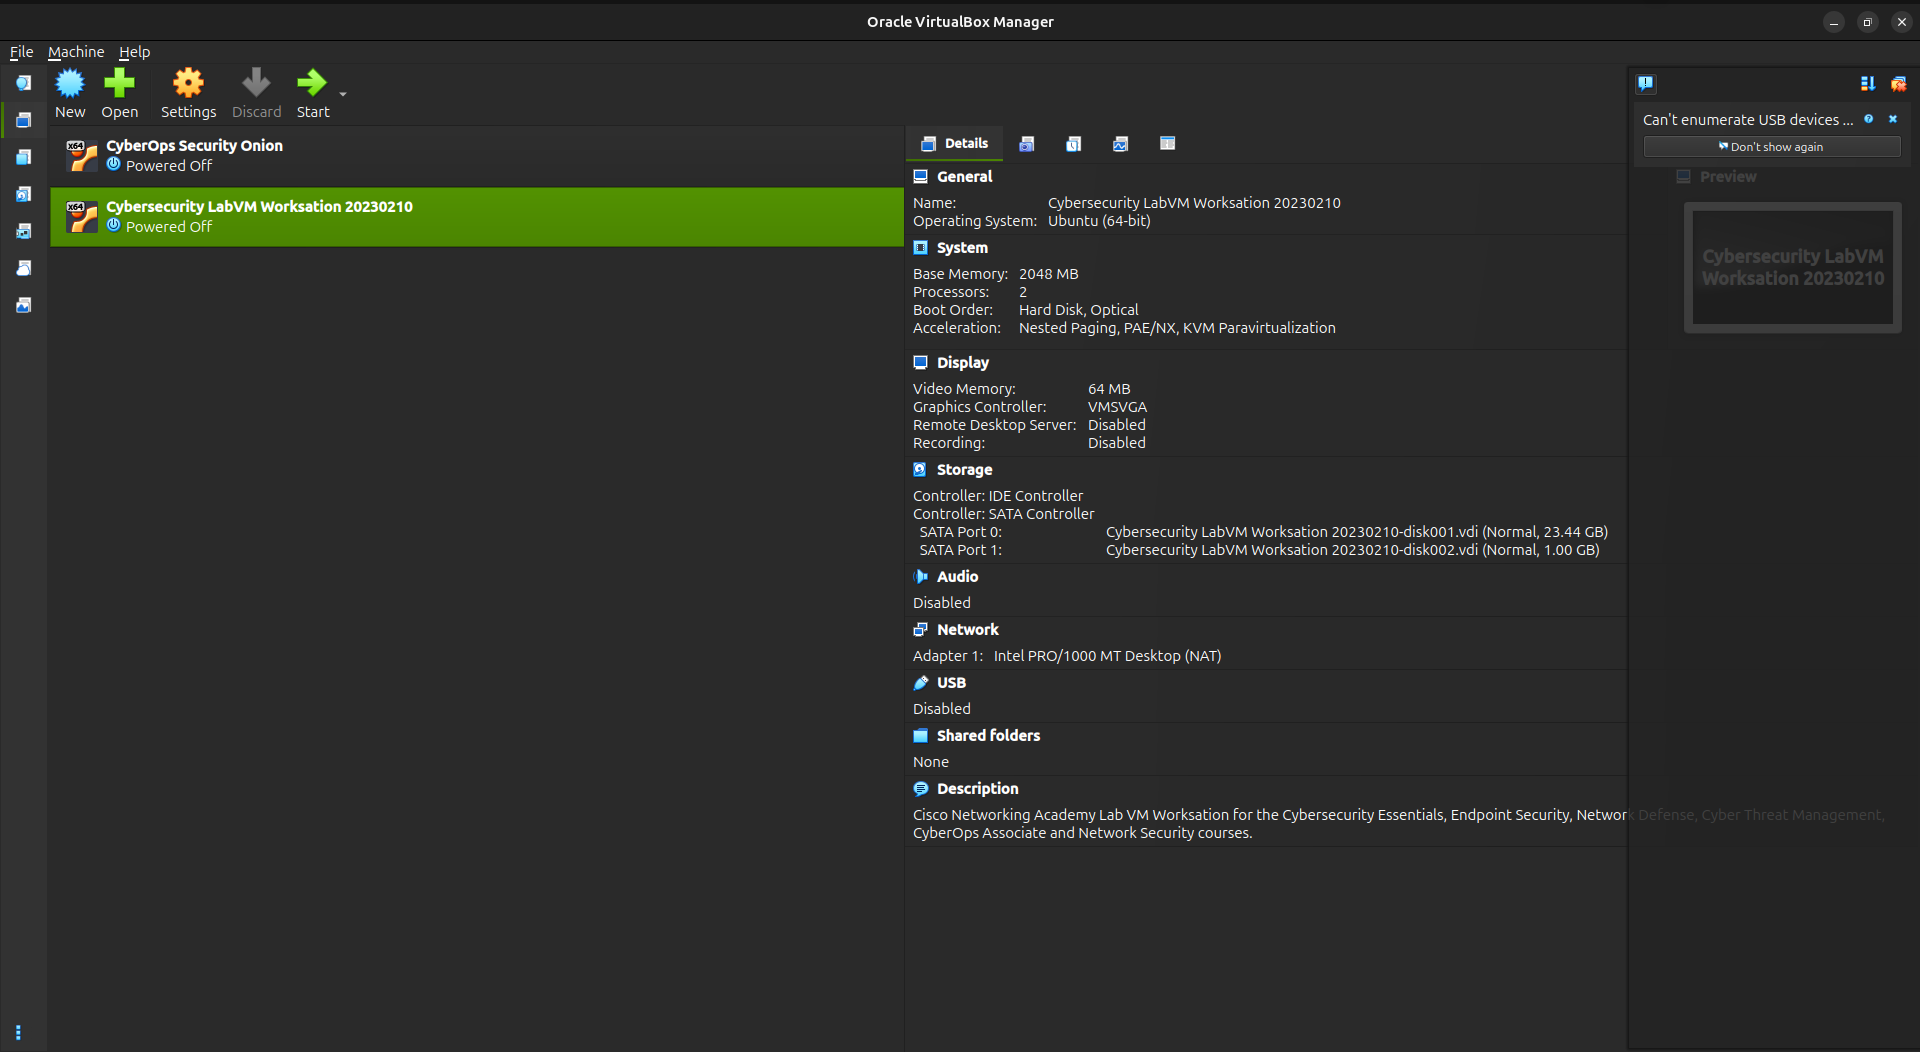
\includegraphics[width=\textwidth]{Pasted image.png}
    \caption{Inventario de VirtualBox con las dos máquinas importadas. La
    estación Cybersecurity LabVM Workstation está seleccionada y se muestra su
    configuración de recursos, almacenamiento y red NAT.}
    \label{fig:inventario}
\end{figure}

\subsection{Configuración de red y acceso a la estación}

La estación \emph{Cybersecurity LabVM Workstation 20230210} tiene habilitado
el primer adaptador de red en modo NAT. Su configuración persistente conserva
la interfaz \texttt{enp0s3} activa con la dirección \texttt{10.0.2.15/24}; el
registro de VirtualBox también muestra tráfico recibido y transmitido en ese
adaptador. Por tanto, la respuesta a la consulta de \texttt{ip address} para la
interfaz de red de la estación es:

\begin{verbatim}
enp0s3: 10.0.2.15/24
\end{verbatim}

El método de acceso indicado por la guía es seleccionar la estación en
VirtualBox, pulsar \emph{Iniciar} e iniciar sesión con el usuario
\texttt{analyst} y la contraseña \texttt{cyberops}. El entorno esperado incluye
los accesos a mostrar escritorio, terminal, administrador de archivos, Firefox,
búsqueda de archivos y directorio personal. Las herramientas específicas del
curso se ubican en \emph{Menú de aplicaciones $>$ CyberOPs}.

La Figura~\ref{fig:workstation-login} confirma que la Workstation inició y
presenta los perfiles disponibles. Para esta práctica corresponde el perfil
\emph{SOC Analyst (CyberOps Associate)}, cuyas credenciales coinciden con las
indicadas por la consigna: \texttt{analyst}/\texttt{cyberops}.

\begin{figure}[H]
    \centering
    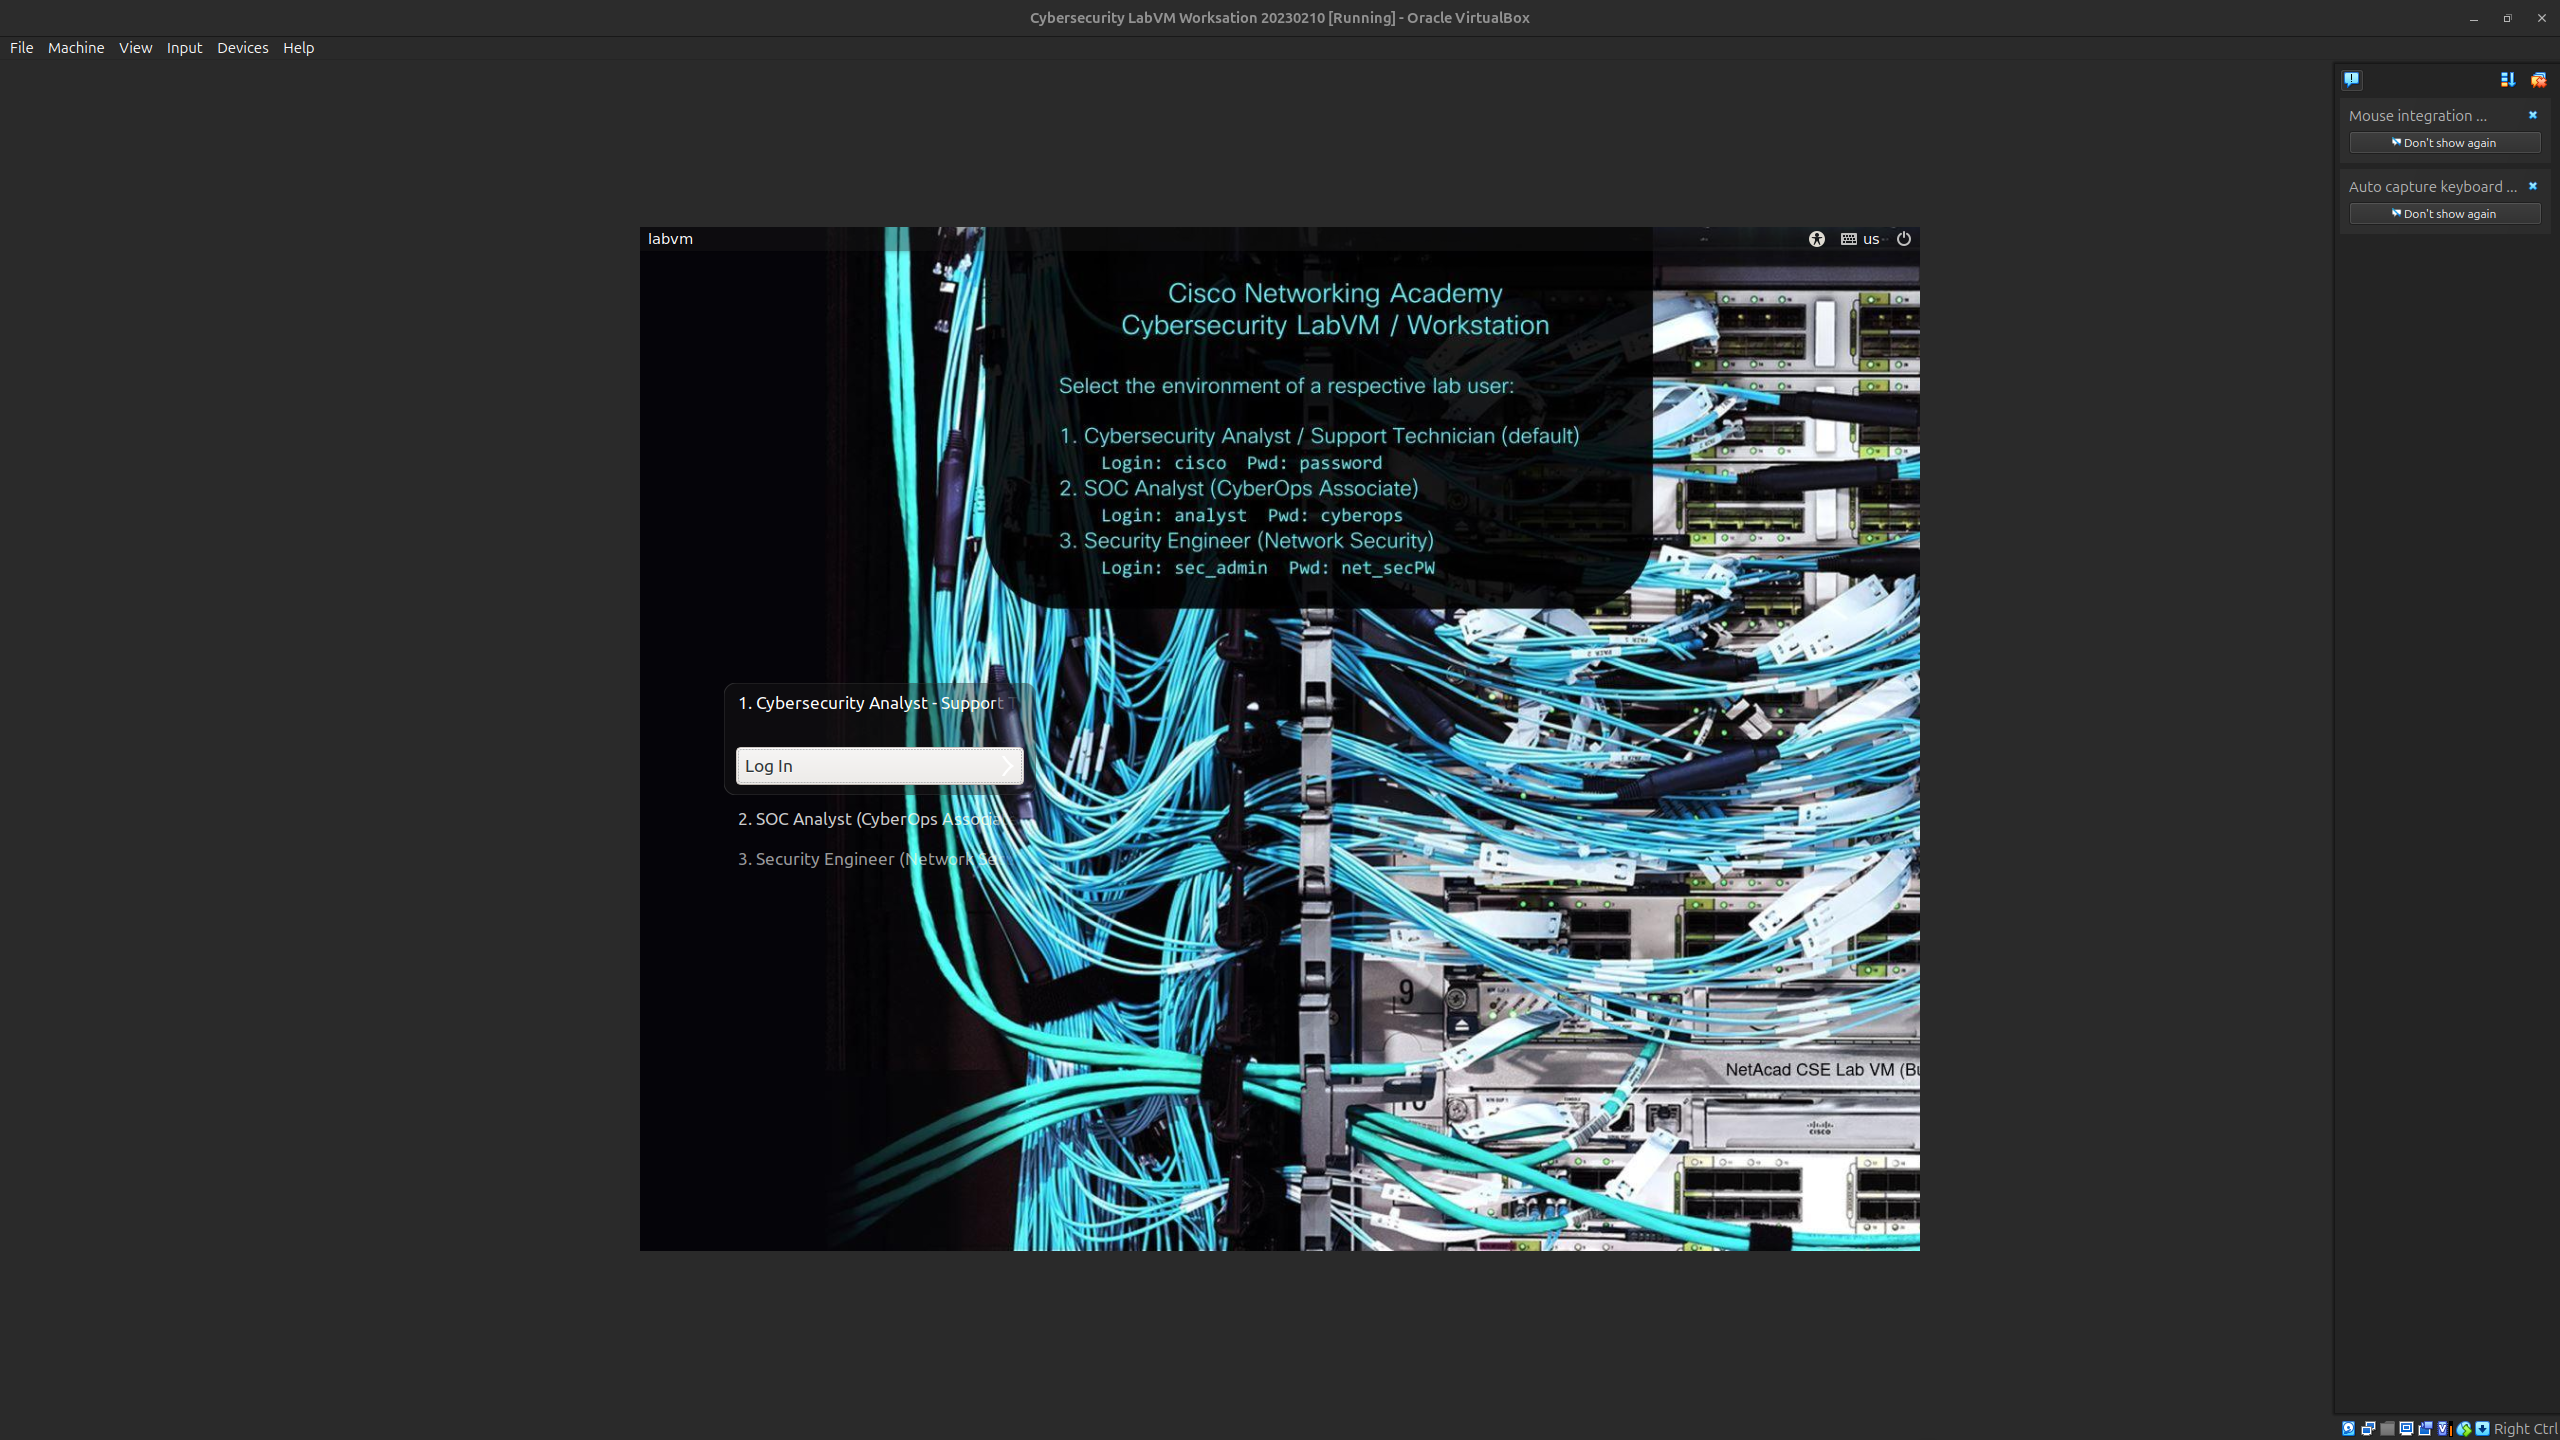
\includegraphics[width=0.92\textwidth]{Pasted image (2).png}
    \caption{Workstation CyberOps en ejecución. La pantalla de selección
    identifica el perfil SOC Analyst y las credenciales requeridas para el
    laboratorio.}
    \label{fig:workstation-login}
\end{figure}

\subsection{Inicio de CyberOps Security Onion}

También se inició \emph{CyberOps Security Onion}, confirmando que la segunda
imagen importada alcanza su pantalla de autenticación. Esta máquina se empleará
en las prácticas que requieren servicios de monitoreo y análisis de seguridad.
La Figura~\ref{fig:security-onion-login} constituye la evidencia de arranque
de la segunda VM.

\begin{figure}[H]
    \centering
    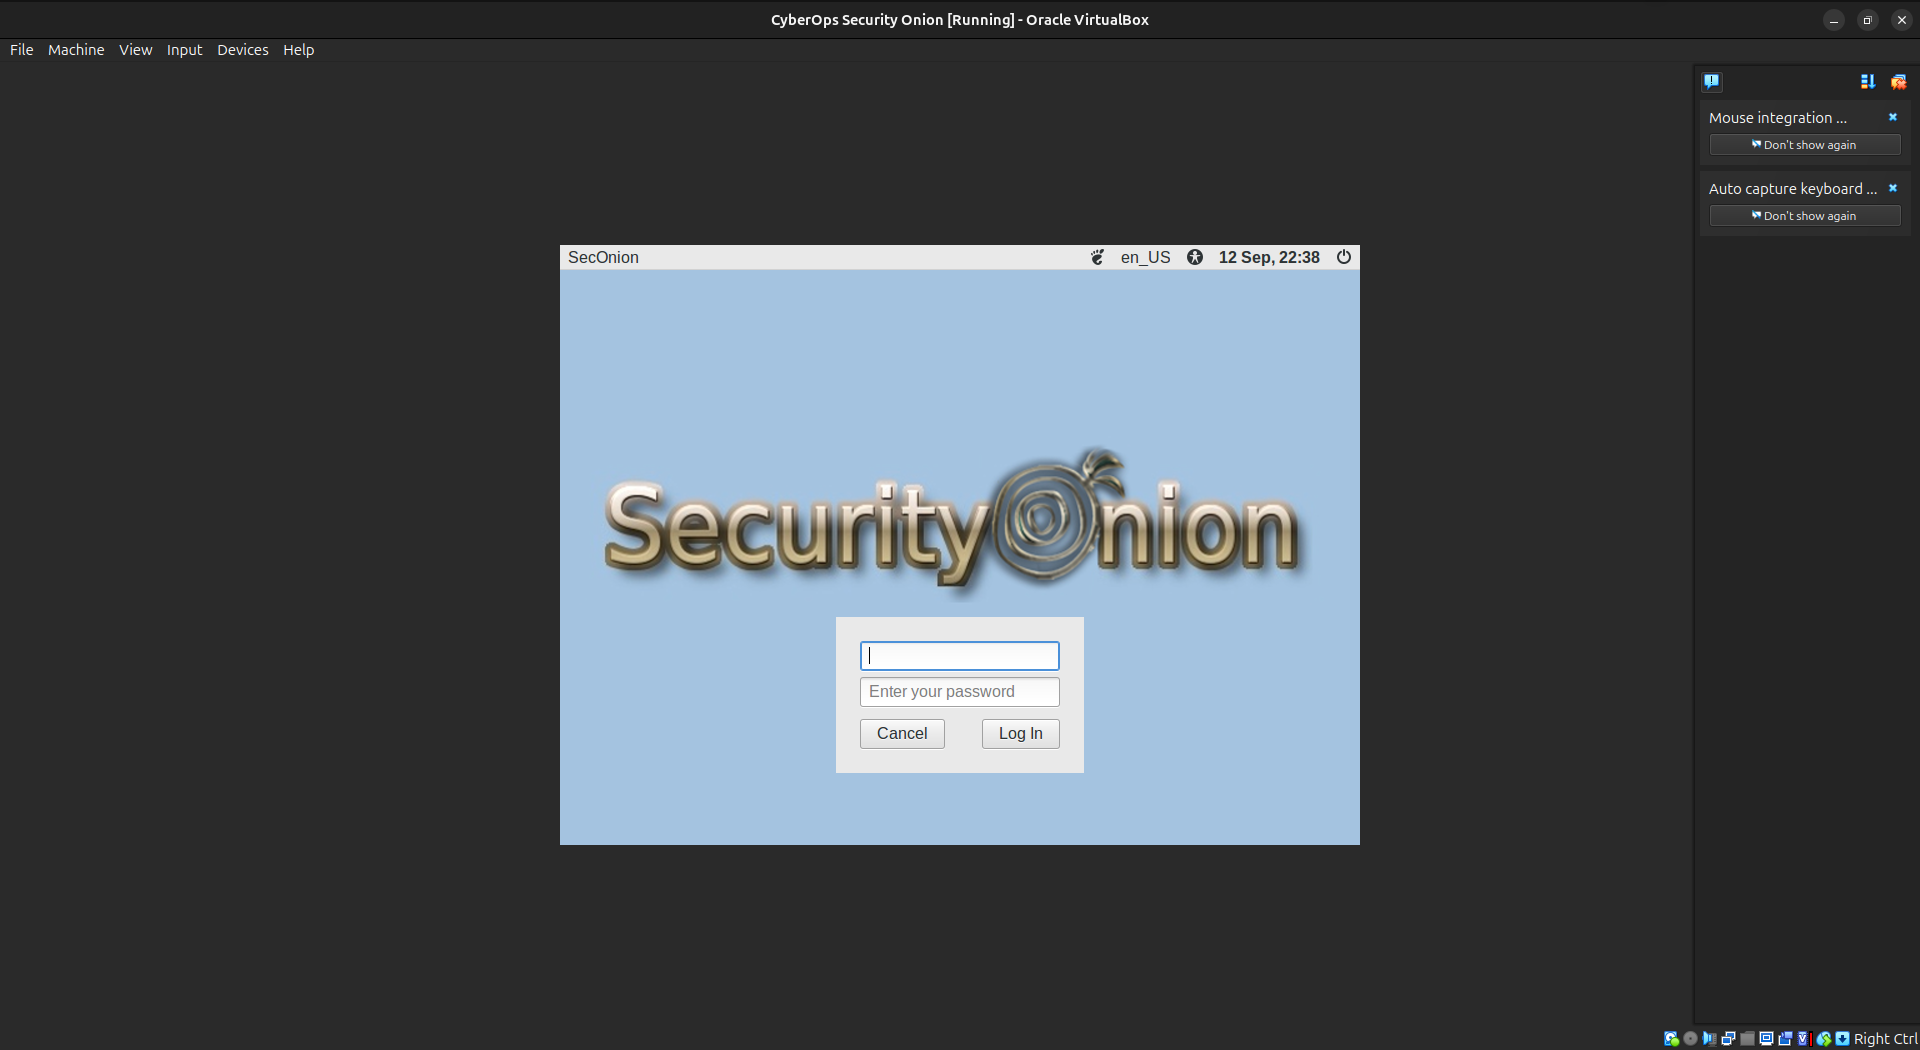
\includegraphics[width=0.9\textwidth]{Pasted image (3).png}
    \caption{Pantalla de autenticación de CyberOps Security Onion en ejecución
    dentro de VirtualBox.}
    \label{fig:security-onion-login}
\end{figure}

\subsection{Cierre seguro}

Al finalizar una práctica se puede usar \emph{Archivo $>$ Cerrar} y seleccionar
\emph{Guardar el estado de la máquina}, de modo que la próxima ejecución
continúe desde el mismo punto. Alternativamente, desde el invitado se puede
ejecutar \texttt{sudo shutdown -h now} para un apagado ordenado o
\texttt{sudo reboot} para reiniciarlo. Se evita la opción de apagar forzosamente
salvo que el sistema no responda, ya que equivale a retirar la alimentación de
una computadora física.

\section{Resultados y respuestas}

La importación de ambas imágenes se encuentra completada y comprobada mediante
el registro de VirtualBox, los discos VDI creados y la Figura~\ref{fig:inventario}.
Las Figuras~\ref{fig:workstation-login} y~\ref{fig:security-onion-login}
evidencian que ambas máquinas inician correctamente. La estación de trabajo
está configurada con NAT y su última dirección IPv4 registrada es
\texttt{10.0.2.15}.

\section{Reflexión}

Una máquina virtual facilita trabajar con entornos aislados, reproducibles y
fácilmente recuperables. Es especialmente útil en ciberseguridad: una práctica
o una herramienta potencialmente riesgosa queda contenida en el invitado y se
puede guardar un estado previo antes de experimentar. Además, permite disponer
de varias configuraciones de red y sistemas operativos en el mismo equipo.

Como contrapartida, las máquinas virtuales consumen memoria, almacenamiento y
capacidad de CPU del anfitrión. Su funcionamiento depende del hipervisor y de
sus módulos de sistema, como evidencia la incidencia de \texttt{vboxdrv}
detectada durante esta práctica. También pueden ofrecer menor rendimiento que
el hardware nativo y requieren configurar cuidadosamente la red para no
exponer servicios de laboratorio de forma involuntaria.

\section{Conclusiones}

Se verificó que los dos OVA proporcionados por el curso están disponibles y
que ya fueron incorporados correctamente a VirtualBox: \emph{Cybersecurity
LabVM Workstation} y \emph{CyberOps Security Onion}. La primera conserva la
configuración NAT solicitada y una dirección asignada de \texttt{10.0.2.15}.
Las capturas incorporadas documentan el inventario, la configuración de la
Workstation y el inicio de ambas máquinas. 
\end{document}
